\documentclass[12pt,a4paper]{article}
\usepackage{geometry}
\usepackage{titlesec}
\usepackage{hyperref}
\usepackage{longtable}
\usepackage{graphicx}

\geometry{margin=1in}
\titleformat{\section}{\bfseries\Large}{\thesection}{1em}{}
\titleformat{\subsection}{\bfseries\normalsize}{\thesubsection}{1em}{}

\title{Functional Design Specification (FDS)}
\author{Project Team Name}
\date{\today}

\begin{document}
	\maketitle
	\tableofcontents
	\newpage
	
	\section{Document Control}
	\begin{tabular}{|l|l|}
		\hline
		Document Title & PsychrometricSolver Functional Design Specification \\
		\hline
		Project Name & PsychrometricSolver \\
		\hline
		Version & 1.0 \\
		\hline		
		Author & Mike Stephenson \\
		\hline
		Approved by & Mike Stephenson \\
		\hline		
		Date & \today \\
		\hline
	\end{tabular}
	
	\section{Introduction}
	\subsection{Purpose}
	 This document defines the functional requirements for the PsychrometricSolver desktop and tablet application. It performs standard psychrometric calculations.
	
	\subsection{Scope}
	Outline the scope of the system or product. 
	
	\subsection{References}
	List relevant standards, regulations, or other documents. 
	
	\section{System Overview}
	Provide a high-level description of the system, its boundaries, and main components. 
	
	\section{Functional Requirements}
	\subsection{Requirement 1}
	\begin{itemize}
		\item \textbf{Description:} The system shall...
		\item \textbf{Inputs:} Data sources, user input, etc.
		\item \textbf{Processing:} Business logic or rules.
		\item \textbf{Outputs:} Results, reports, UI response.
	\end{itemize}
		
	\begin{figure}[h]
		\centering
		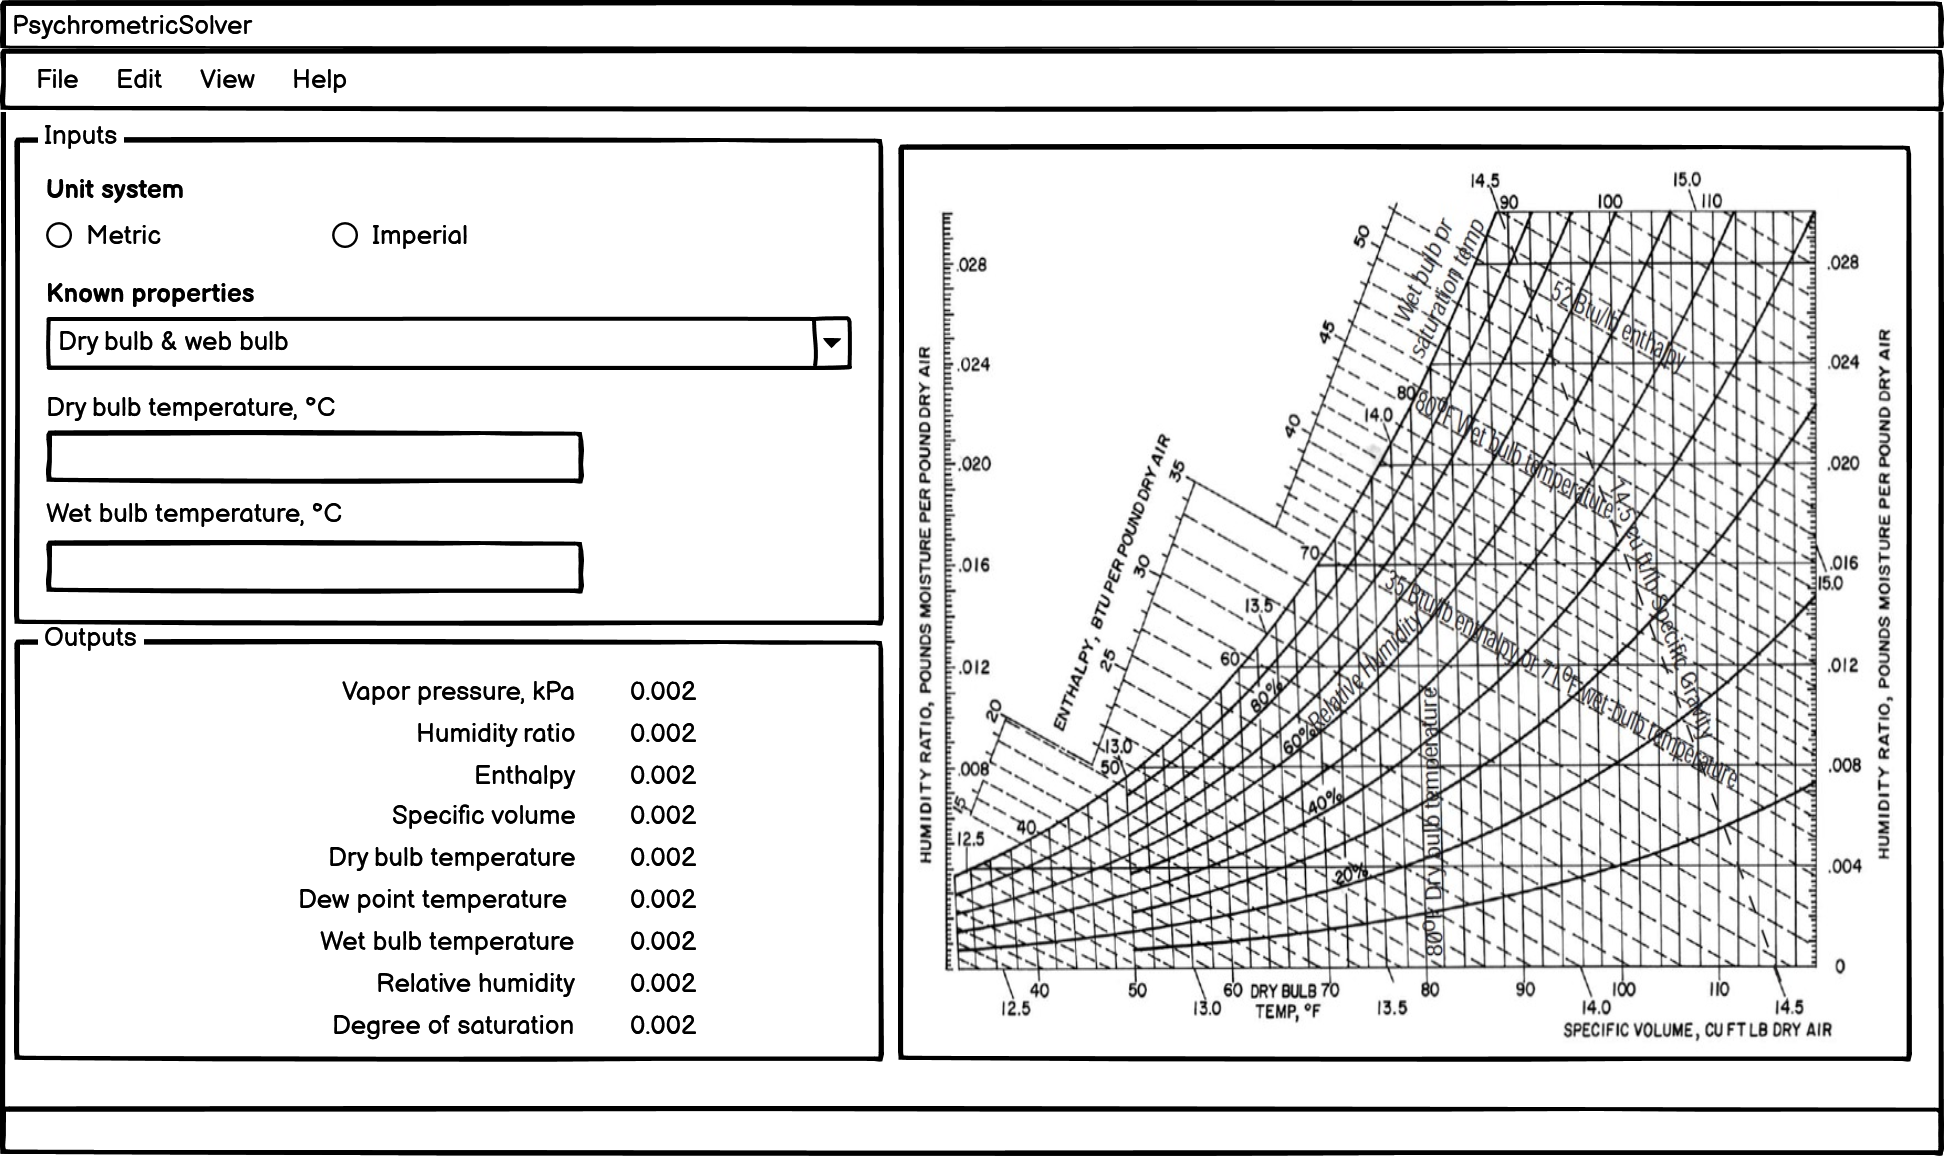
\includegraphics[width=0.85\textwidth]{psychrometic-solver-main-screen.png}
		\caption{Main Screen.}
	\end{figure}
		
	\subsection{Requirement 2}
	Repeat for each functional requirement.
	
	\section{System Functions}
	\begin{longtable}{|p{3cm}|p{10cm}|}
		\hline
		\textbf{Function ID} & F-001 \\
		\hline
		\textbf{Name} & User Login \\
		\hline
		\textbf{Description} & Allow a registered user to log in securely. \\
		\hline
		\textbf{Inputs} & Username, Password \\
		\hline
		\textbf{Processing Rules} & Validate credentials, check lockout status. \\
		\hline
		\textbf{Outputs} & Login success/failure message \\
		\hline
	\end{longtable}
	
	\section{Performance Requirements}
	Define response times, throughput, capacity, and accuracy requirements.
	
	\section{Constraints}
	List compliance, hardware/software dependencies, environmental requirements.
	
	\section{Acceptance Criteria}
	Specify how each function will be validated and tested. 
	
	\section{Appendices}
	Glossary, diagrams, or supporting documentation. 
	
\end{document}
